\documentclass[11pt, letterpaper]{article}
\usepackage[utf8]{inputenc}
\usepackage[margin=1in]{geometry}
\usepackage{enumitem}
\usepackage{indentfirst}
\usepackage{titling}
\usepackage{graphicx}
\usepackage{amsmath}
\usepackage{amsfonts}
\usepackage{mathtools}
\usepackage{hyperref}
\usepackage{mathabx}
\usepackage{caption}
\usepackage{subcaption}
\usepackage{bm}
\usepackage{textcomp}
\graphicspath{ {./} }
\DeclareMathAlphabet{\altmathcal}{OMS}{cmsy}{m}{n}

\newcommand{\bv}[2][]{\bm{\vec{#2}_{#1}}}

\setlength{\parindent}{0cm}
\setlength{\parskip}{1em}
\renewcommand{\baselinestretch}{1.5}

\hypersetup{
    colorlinks=true,
    linkcolor=cyan,
    filecolor=magenta,      
    urlcolor=blue,
}

\title{Chapter VI: Capacitors and Dielectrics}
\author{Chenyi Zhu}
\date{March 24th, 2020}

\begin{document}


\begin{titlingpage}
	\maketitle
	
	\begin{center}
		Look on the bright side. :)
	\end{center}
	
	\begin{figure}[h!]
		\centering
		
\includegraphics[scale=0.2]{tweet}
		\label{fig:flux}
	\end{figure}
		
\end{titlingpage}
	
\section{Introduction.}
A capacitor, consisted of two parallel plates of equal but opposite charge, stores electric charge. When \textit{uncharged}, the charge on either one of the conductors in the capacitor $ = 0\, C$. The simplest example is a set of parallel plates each of area $A$, separated by $d$. 
\begin{figure}[h!]
	\centering
	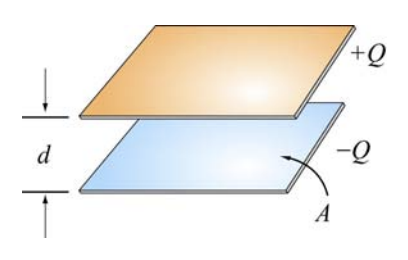
\includegraphics[scale=0.8]{simple-capacitor.png}
	\caption{Simple capacitor.}
	\label{fig:simple-capacitor}
\end{figure}

Experiments have shown that the amount of charge $Q$ is linearly proportional to $\Delta V$:
\begin{equation}\label{eqn:capacitance}
	\boxed{Q = C\,|\Delta V|}
\end{equation}
where we call $C$ \textbf{capacitance}. Physically, capacitance is a measure of capacity of storing electric charge for a given potential difference $\Delta V$. The SI unit of capacitance is the \textit{farad}($F$): \[1\, F = 1\, farad = 1\, C/V\] \textbf{Note}: a typical capacitance ranges from the picofarad ($1\, pF = 10^{-12}\, F$) to millifarad ($1\, mF = 10^{-3}\, F$). 

\section{Calculations.}
Here we will find formulae for capacitance for some typical geometries.

\textbf{Example 1}. Consider two metallic plates of equal area $A$ separated by a distance $d$, as shown below. The top plate carries a charge $+Q$ while the bottom carries a charge $-Q$. The capacitor is charged with a battery (no need to know the voltage of this battery). Find the capacitance. 
\begin{figure}[h!]
	\centering
	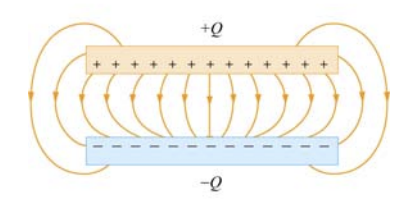
\includegraphics[scale=1]{eg1.png}
	\caption{Electric field between two parallel plates.}
	\label{fig:eg1}
\end{figure}

\textbf{Solution}. To find the capacitance, we first need to consider the electric field produced by the plates.

\textbf{Note}: in real life the capacitor plates are finite, and therefore there will always be \textit{edge effects} which refer to the electric field lines near the edge of the capacitor that are not straight lines, and the non-uniform fields near the edge are called the ``fringing fields''. Although in the figure above we showed the edge effects, we will ignore it for the sake of simplicity for the rest of the problem. 

Take $\lim_{A\to\infty}$, we would have a system with planar symmetry and we can calculate $\bv{E}$ everywhere with Gauss's Law: \[\oiint_S \bv{E}\cdot\, d\bv{A} = \frac{q_{enc}}{\varepsilon_0}\] Now we choose a Gaussian ``pillbox'' with cap area $A'$ to enclose the charge on the \textbf{positive} plate. 
\begin{figure}[h!]
	\centering
	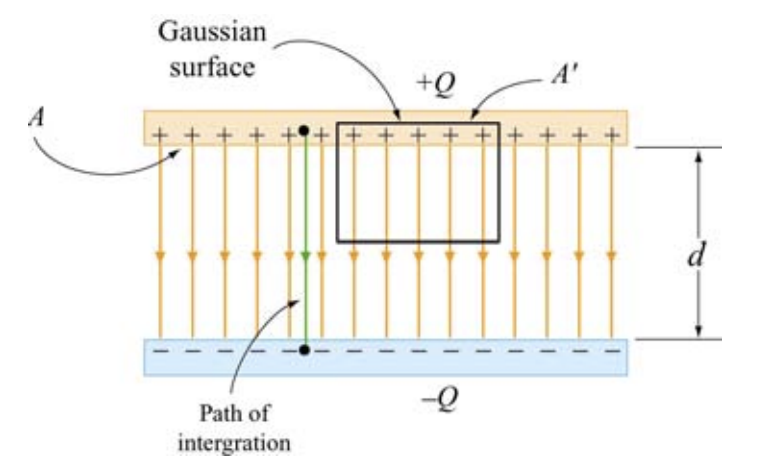
\includegraphics[scale=0.5]{gauss.png}
	\caption{Gaussian ``pillbox'' encloses charge.}
	\label{fig:gauss}
\end{figure}

The electric field in the region between the plates is \[EA' = \frac{q_{enc}}{\varepsilon_0} = \frac{\sigma A'}{\varepsilon_0}\Rightarrow E = \frac{\sigma}{\varepsilon_0}\] and the potential difference between the plates follow: \[\Delta V = V_- - V_+ = -\int_+^-\bv{E}\cdot\, d\bv{s} = -Ed\] where we take the straight field lines as the path of integration to preserve the correct sign. However, we don't really care about signs in calculating capacitance, so we just take the magnitude of the potential difference: \[\Delta V= Ed\] and from the definition of capacitance,
\begin{equation}
	\boxed{C = \frac{Q}{|\Delta V|} = \frac{\varepsilon_0 A}{d} \text{ (for paralell plates)}}
\end{equation}

\section{Capacitors in Electric Circuits.}
\subsection{Capacitors in Parallel}
Consider a system with a battery with potential difference $\Delta V$ and $n$ capacitors connected in parallel with capacitance $C_1, C_2,...,C_n$. 
\begin{figure}[h!]
	\centering
	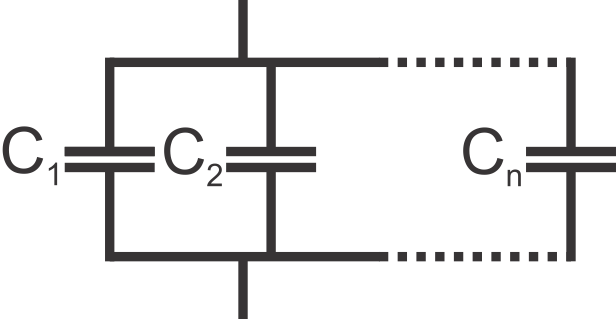
\includegraphics[scale=0.2]{parallel.png}
	\caption{$n$ capacitors connected in parallel.}
	\label{fig:parallel}
\end{figure}

The equivalent capacitance of all the capacitors is thus
\begin{equation}\label{eqn:parallel}
	\boxed{C_{eq} = \sum_{i = 1}^{n}C_i}
\end{equation}
Each capacitor has the same potential difference $\Delta V$ in this configuration, but not the same amount of charge.

\subsection{Capacitors in Series.}
Consider a system with the same battery and $n$ capacitors connected in series with capacitance $C_1, C_2,...,C_n$.
\begin{figure}[h!]
	\centering
	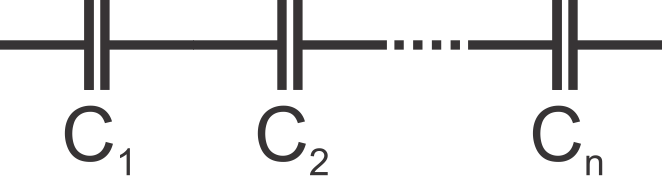
\includegraphics[scale=0.2]{series.png}
	\caption{$n$ capacitors connected in series.}
\end{figure}

The equivalent capacitance of all the capacitors is 
\begin{equation}\label{eqn:series}
	\boxed{\frac{1}{C_{eq}} = \sum_{i = 1}^{n}\frac{1}{C_i}}
\end{equation}
Each capacitor has the same charge $Q$, but not the same potential difference.

\section{Storing Energy.}
As you have learned, capacitors can store electric energy. The amount of energy stored is equal to the work done to charge it. During the charging process, the battery does work to removed charges from one plate and deposit them onto the other. 
\begin{figure}[h!]
	\centering
	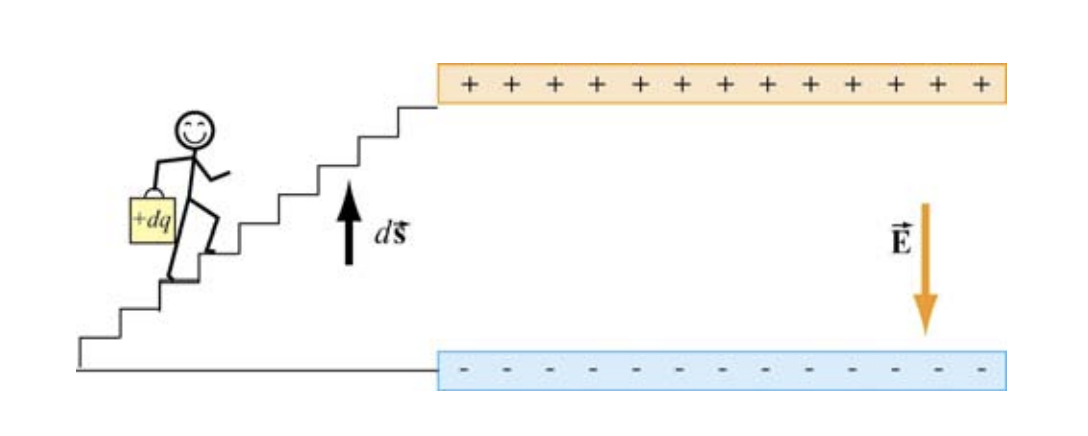
\includegraphics[scale=0.5]{man.png}
	\caption{Work done to bring $dq$ from bottom to top plate.}
	\label{fig:man}
\end{figure}

Suppose the amount of charge on the top t some instance is $+q$, and the potential difference between the two plates is $|\Delta V| = q/C$. To add another charge of $dq$ on the top plate, the amount of work done to overcome electrical repulsion is $dW = |\Delta V|dq$. If at the end the charge on the top plate is $+Q$, then the total amount of work done in the process is \[W = \int_0^Q dq\, |\Delta V| = \int_0^Q dq\, \frac{q}{C} = \frac{Q^2}{2C}\] which is equal to the electrical potential energy $U_E$ of the system:
\begin{equation}\label{eqn:energy}
	\boxed{U_E = \frac{Q^2}{2C} = \frac{Q|\Delta V|}{2} = \frac{C|\Delta V|^2}{2}}
\end{equation}
\textbf{Note}: $q$ is used as a variable to integrate over, while $Q$ is a constant.

\subsection{Energy Density}
Think of energy stored in the capacitor as the energy stored in the electric field itself. In the case of a parallel capacitor, we have: \[U_E = \frac{C|\Delta V|^2}{2} = \frac{1}{2}\frac{\varepsilon_0 A}{d}(Ed)^2 = \frac{1}{2}\,\varepsilon_0 E^2(Ad)\] and since $Ad$ represents precisely the volume enclosed by the two plates, we can define electric energy density as
\begin{equation}\label{eqn:energy-density}
	\boxed{u_E = \frac{U_E}{volume} = \frac{1}{2}\varepsilon_0 E}
\end{equation}
where $u_E$ is proportional to the square of the electric field. 

\section{Dielectrics.}
In many capacitors there is an insulating material such as paper or plastic between the plates. Such material, called a \textbf{dielectric}, can be used to maintain a physical separation of the plates. Since dielectrics break down less readily than air, charge leakage can be minimized, especially when high voltage is applied.

Experimentally it was found that capacitance increases when the space between the conductors is filled with dielectrics. Suppose a capacitor has a capacitance $C_0$ when the space between the plates is vacuum. When a dielectric material is inserted to completely fill the space between the plates, the capacitance would change to \[C = \kappa_e C_0\] where $\kappa_e$ is the \textbf{dielectric constant}. Dielectric constant of a material is then defined as the ratio of its \textbf{permittivity} and \textbf{permittivity of vacuum} $\varepsilon_0$, so \[\kappa = \frac{\varepsilon}{\varepsilon_0}\] Experiments indicate that all dielectric materials have $\kappa_e > 1$.

\textbf{Note}: Every dielectric material has a \textit{characteristic dielectric strength} which is the maximum value of electric field before breakdown occurs and charges begin to flow. 

The fact that capacitance increases with the presence of a dielectric can be explained from a molecular point of view. We shall show that $\kappa_e$ is a measure of the dielectric response to an eternal electric field. There are two types of dielectrics: \textbf{polar} (which have permanent electric dipole moments) and \textbf{non-polar} (which do not have the permanent dipole moments).  
\begin{figure}
	\centering
	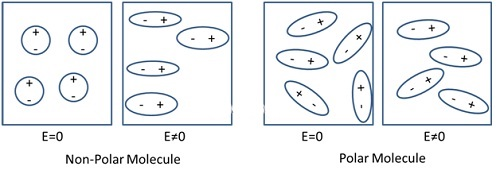
\includegraphics[scale=0.5]{polar.jpg}
	\caption{Polar and non-polar dielectrics, $\bv{E}$ points from left to right.}
	\label{fig:polar}
\end{figure}

With polar molecules, the orientation is random without an external field. When the field is applied, however, the alignment is not perfect due to random thermal motion. The aligned molecules can generate an electric field that is opposite to the applied field but smaller in magnitude. With non-polar molecules, applying an external field will ``induce'' a charge on the molecules' surfaces in the opposite direction. 

\subsection{Gauss's Law for Dielectrics}
From \hyperref[fig:gauss]{this} previous example we saw that, without any dielectrics, the electric field $\bv[0]{E}$ in the region between the plates can be found by using Gauss's Law: \[\oiint_S\bv{E}\cdot\, d\bv{A} = E_0A = \frac{Q}{\varepsilon_0}\Rightarrow E_0 = \frac{\sigma}{\varepsilon_0} \] We have seen that when a dielectric is inserted, there is an induced charge $Q_P$ of opposite sign on the surface, and the net charge enclosed by the Gaussian surface is $Q - Q_P$. 
\begin{figure}[h!]
	\centering
	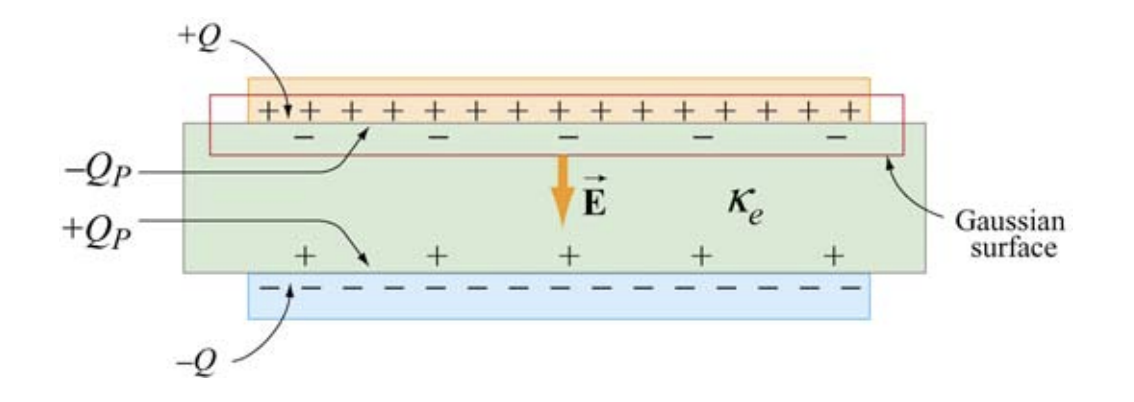
\includegraphics[scale=0.4]{dielectric.png}
	\caption{Gauss's Law for capacitor with dielectrics.}
	\label{fig:dielectric}
\end{figure}

Gauss's Law now becomes: \[\oiint_S\bv{E}\cdot\, d\bv{A} = EA = \frac{Q- Q_P}{\varepsilon_0}\] or 
\begin{equation}
	\boxed{E = \frac{Q - Q_P}{\varepsilon_0 A}}
\end{equation}
But we have just seen that the effect of the dielectric is to weaken the original field $E_0$ by a factor $\kappa_e$: \[E = \frac{E_0}{\kappa_e} = \frac{Q}{\kappa\varepsilon_0A} = \frac{Q - Q_P}{\varepsilon_0A}\] from which the induced charge $Q_P$ can be obtained as \[Q_P = Q\left(1 - \frac{1}{\kappa_e}\right)\] In terms of the surface charge density, we have \[\sigma_P = \sigma \left(1 - \frac{1}{\kappa_e}\right)\] Note that in the limit $\kappa_e = 1$, $Q_P = 0$ which corresponds to the case of vacuum. \[\oiint_S \bv{E}\cdot\, d\bv{A} = \frac{Q}{\kappa_e\varepsilon_0} = \frac{Q}{\varepsilon}\] Alternatively, we may also write \[\oiint_S\bv{D}\cdot\, d\bv{A} = Q\] where $\bv{D} = \varepsilon_0\kappa\bv{E}$ is called the electric displacement vector.

\section{Appendix.}
\subsection{Problem Solving Strategies}
To find the capacitance of a given geometry:
\begin{itemize}
	\item Identify the direction of the electric field using symmetry;
	\item Calculate electric field everywhere;
	\item Compute the electric potential difference $\Delta V$.
\end{itemize}
\subsection{Capacitance of Different Geometries}
\begin{table}[h!]
	\centering
	\begin{tabular}{||c|c||}
	\hline
	\textbf{System} & \textbf{Capacitance}\\
	\hline
	Isolated charged sphere of radius $R$ & $C = 4\pi\varepsilon_0R$\\
	\hline
	Parallel-plate capacitor of plate area $A$ and plate separation $d$ & $C = \varepsilon_0\frac{A}{d}$\\
	\hline
	Cylindrical capacitor of length $L$, inner radius $a$ and outer radius $b$ & $C = \frac{2\pi\varepsilon_0L}{ln(b - a)}$\\
	\hline
	Spherical capacitor with inner radius $a$ and outer radius $b$ & $C = 4\pi\varepsilon_0\frac{ab}{b - a}$\\
	\hline
	\end{tabular}
	\caption{\label{tbl:geometries}Capacitance of different geometries.}
\end{table}
\subsection{Clarifications}
It is important to remember that capacitors allow \textbf{currents} to flow, not \textbf{electrons} to flow, which is why I used $dq$ in the \hyperref[fig:man]{analogy} to relate to current.

\section{Exercises.}
\subsection{Warm-up}
\textbf{Problem 1}. Derive the capacitance for each of the geometries listed in \hyperref[tbl:geometries]{table 6.1}. 

%5.10.4
\textbf{Problem 2}. Consider an air-filled parallel-plate capacitor with one plate connected to a spring having a force constant $k$, and another plate held fixed. The system rests on a table top. Ignore friction, if the charges placed on plates $a$ and $b$ are $+Q$ and $-Q$ respectively, how much does the spring extend?
\begin{figure}[h!]
	\centering
	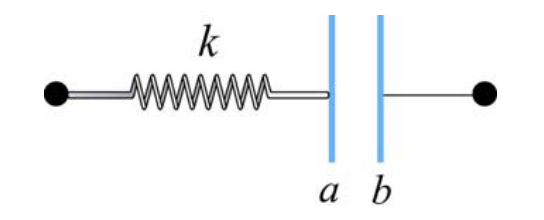
\includegraphics[scale=0.5]{spring.png}
	\caption{Spring attached to capacitor.}
	\label{fig:spring}
\end{figure}

\subsection{Conceptual Questions}
%5.11.1, 2, 4
\textbf{Problem 3}.  The charges on the plates of a parallel-plate capacitor are of opposite sign, and they attract each other. To increase the plate separation, is the external work done positive or negative? What happens to the external work done in this process?

\textbf{Problem 4}. How does the stored energy change if the potential difference across a capacitor is tripled?

\textbf{Problem 5}. If a dielectric-filled capacitor is cooled down, what happens to its capacitance?

\subsection{More Practice}
%e.g 5.7
\textbf{Problem 6}. A non-conducting slab of thickness $t$ , area $A$ and dielectric constant $\kappa_e$ is inserted into the space between the plates of a parallel-plate capacitor with spacing $d$, charge $Q$ and area $A$, as shown below. The slab is not necessarily halfway between the capacitor plates. What is the capacitance of the system?
\begin{figure}[h!]
	\centering
	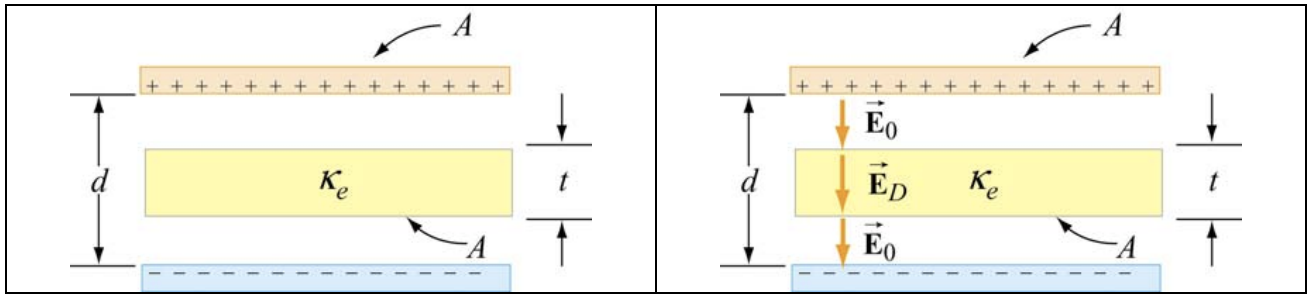
\includegraphics[scale=0.6]{halfway.png}
	\caption{Non-conducting slab inside capacitor.}
	\label{fig:halfway}
\end{figure}

%5.12.7
\textbf{Problem 7}. Consider the case in which a dielectric material with dielectric constant $\kappa_e$ completely fills the space between the plates of a parallel-plate capacitor. Show that the energy density of the field between the plates is $u_E = \frac{\bv{E}\cdot\bv{D}}{2}$ by the following procedure:
\begin{itemize}
	\item Eliminate $\bv{D}$ and write the expression in terms of $\bv{E}$ and $\kappa_e$;
	\item  Given the electric field and potential of such a capacitor with free charge $q$ on it, calculate the work done to charge the capacitor from $q = 0$ to $q = Q$;
	\item Find energy density $u_E$.
\end{itemize}



\end{document}
